\documentclass[usenames,dvipsnames]{beamer}

\mode<presentation> {
    \usetheme{Montpellier}
}

\usepackage{graphicx} % Allows including images
\usepackage[frenchb]{babel}
\usepackage[T1]{fontenc}
\usepackage[utf8]{inputenc}
\usepackage{booktabs} % Allows the use of \toprule, \midrule and \bottomrule in tables
\setcounter{tocdepth}{2}
\graphicspath{{../../Figures/}}


% exercices comptés
\newcounter{numexos}%Création d'un compteur qui s'appelle numexos
\setcounter{numexos}{0}%initialisation du compteur
\newcommand{\exercice}[1]{%Création d'une macro ayant un paramètre
\addtocounter{numexos}{1}%chaque fois que cette macro est appelée, elle ajoute 1 au compteur numexos
\textcolor{DarkOrchid}{Exercice\,\thenumexos\,:}\,#1%Met en rouge Exercice et la valeur du compteur appelée par \thenumeexos
}
%----------------------------------------------------------------------------------------
\setbeamertemplate{title page}{
    \centering

    \Large\bfseries
    Machine learning Tek 5: dimensionality reduction
    

\begin{figure}[!h]
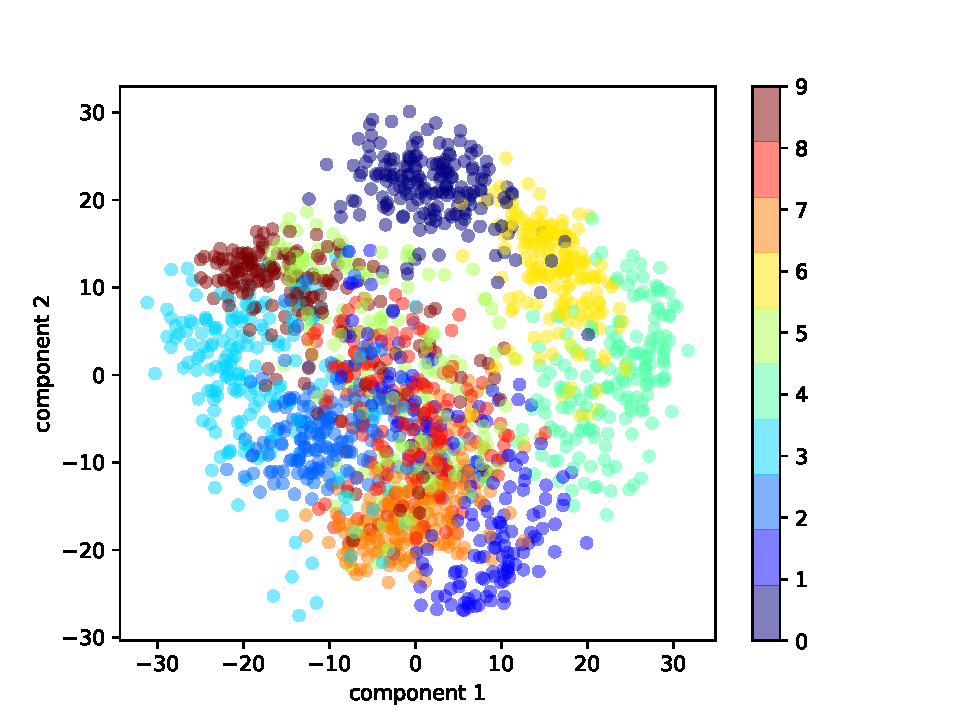
\includegraphics[width=8cm]{projected_digits}
\end{figure}

    }

\begin{document}

\begin{frame}
    \titlepage % Print the title page as the first slide
\end{frame}

\begin{frame}
    \frametitle{Overview} % Table of contents slide, comment this block out to remove it
    \tableofcontents % Throughout your presentation, if you choose to use \section{} and \subsection{} commands, these will automatically be printed on this slide as an overview of your presentation
\end{frame}

\section{Motivation}
\frame{\tableofcontents[currentsection]}

\begin{frame}{Why is the dimension so important ?}
    Recall $2$ important constants in machine leaning:
    \begin{itemize}
        \item $n$: number of samples
        \item $d$: dimension of the samples (number of features)
    \end{itemize}
    The space $ \mathcal{X} $ that contains the data, for either supervised or unsupervised learning is often included in $\mathbb{R}^d$.
\end{frame}

\begin{frame}{Dimensionality reduction}
    \begin{itemize}
        \item $ \mathcal{X}\subset \mathbb{R}^d$.
        \item If $d$ is large (e.g. $\geq 10^4$), the algorithms that run on the data might become too slow to be used, as their algorithmic complexity depends on $d$ (potentially in a quadratic or exponential way, curse of dimensionality)
        \item we will illustrate this problem with local averaging.
    \end{itemize}
\end{frame}

\begin{frame}{Local averaging}

    Local averaging is a prediction method that is not based on any opitmization, but only based on the dataset itself.

    \begin{figure}[htpb]
    	\centering
    	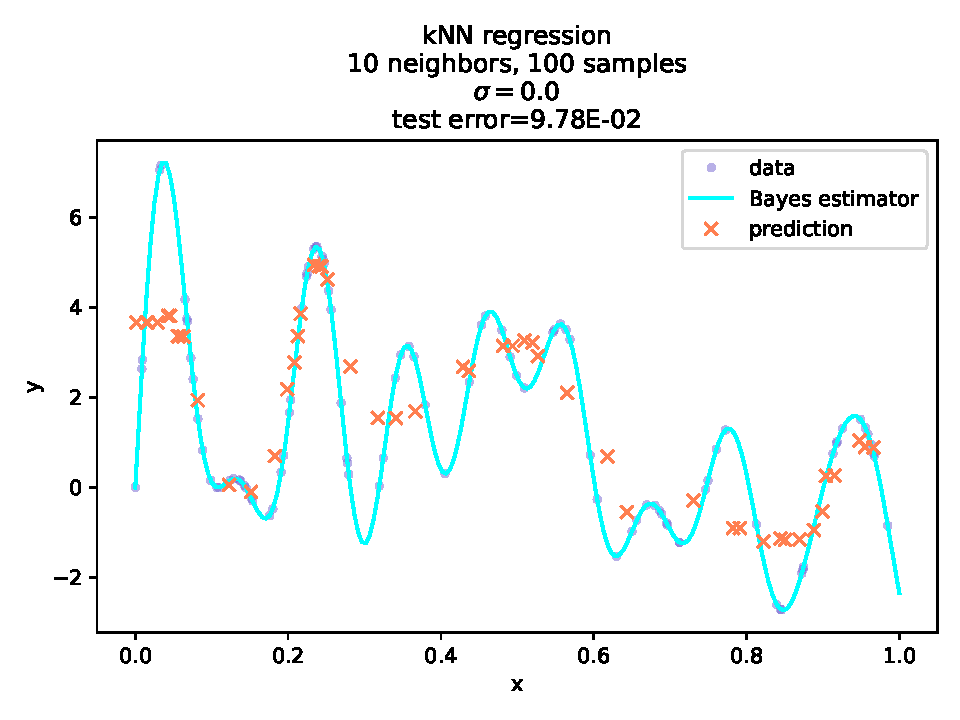
\includegraphics[width=0.6\textwidth]{images_1D/knn_k=10_samples=100_sigma=0}
    	\label{fig:images_1D-knn_k-20_samples-100000_sigma-1}
    \end{figure}
\end{frame}

\begin{frame}
    \begin{figure}[htpb]
    	\centering
    	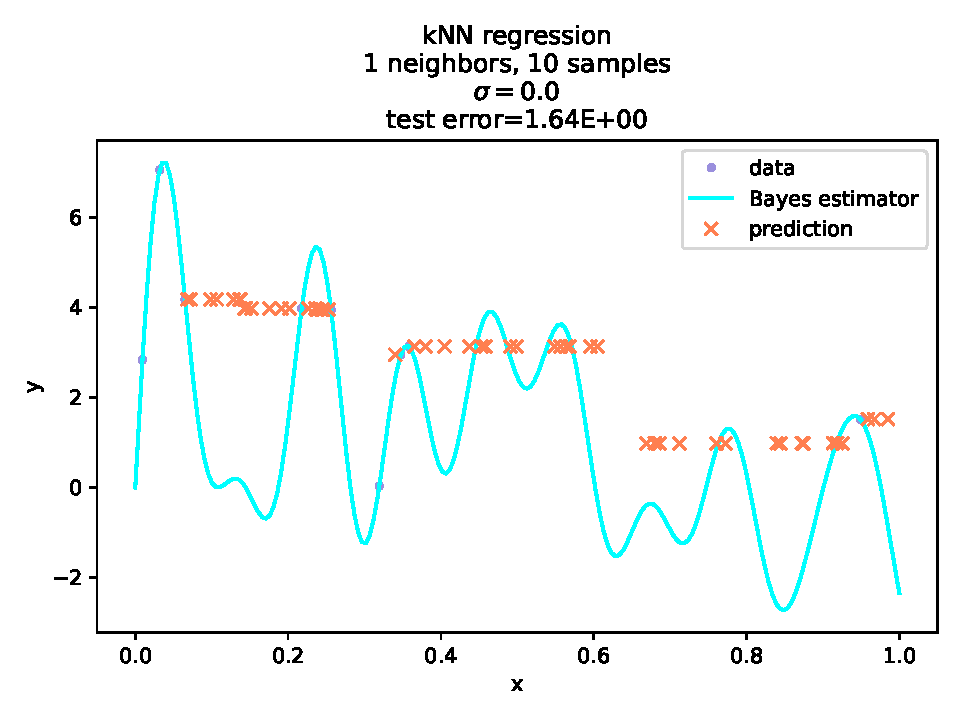
\includegraphics[width=0.7\textwidth]{images_1D/knn_k=1_samples=10_sigma=0}
    	\label{fig:images_1D-kn}
    \end{figure}
\end{frame}

\begin{frame}
    \begin{figure}[htpb]
    	\centering
    	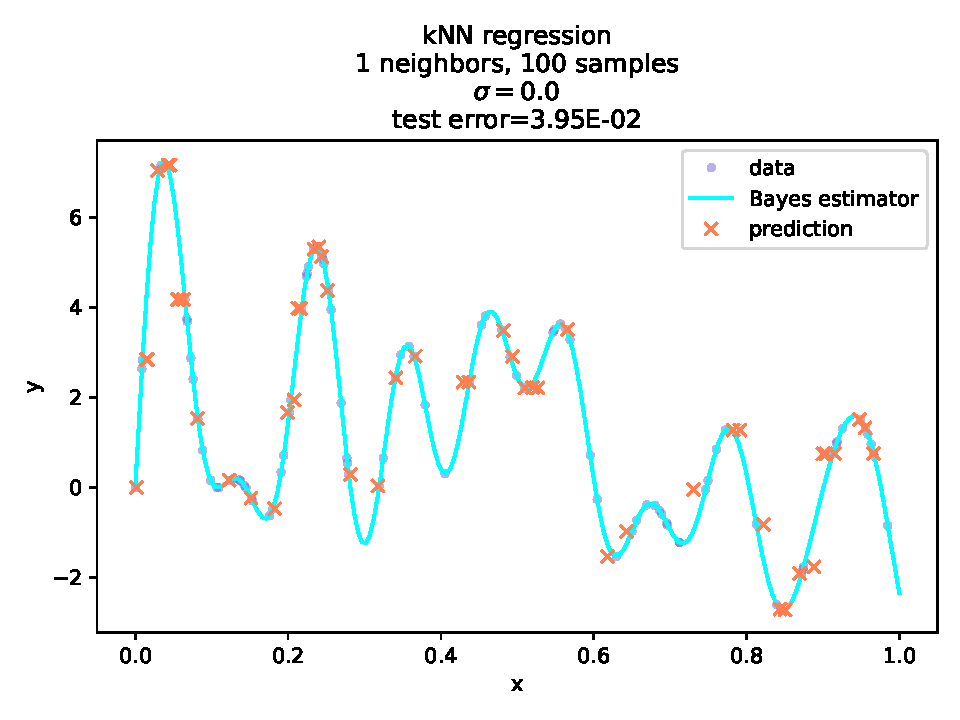
\includegraphics[width=0.7\textwidth]{images_1D/knn_k=1_samples=100_sigma=0}
    	\label{fig:images_1D-kn}
    \end{figure}
\end{frame}


\begin{frame}
    \begin{figure}[htpb]
    	\centering
    	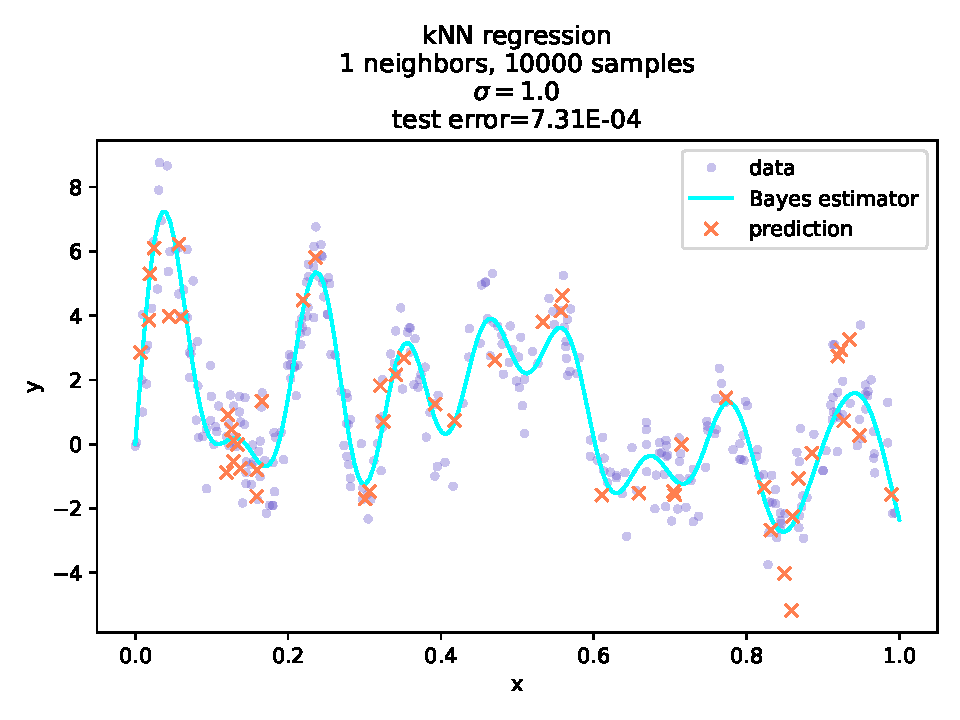
\includegraphics[width=0.7\textwidth]{images_1D/knn_k=1_samples=10000_sigma=1}
    	\label{fig:images_1D-kn}
    \end{figure}
\end{frame}

\begin{frame}
    \begin{figure}[htpb]
    	\centering
    	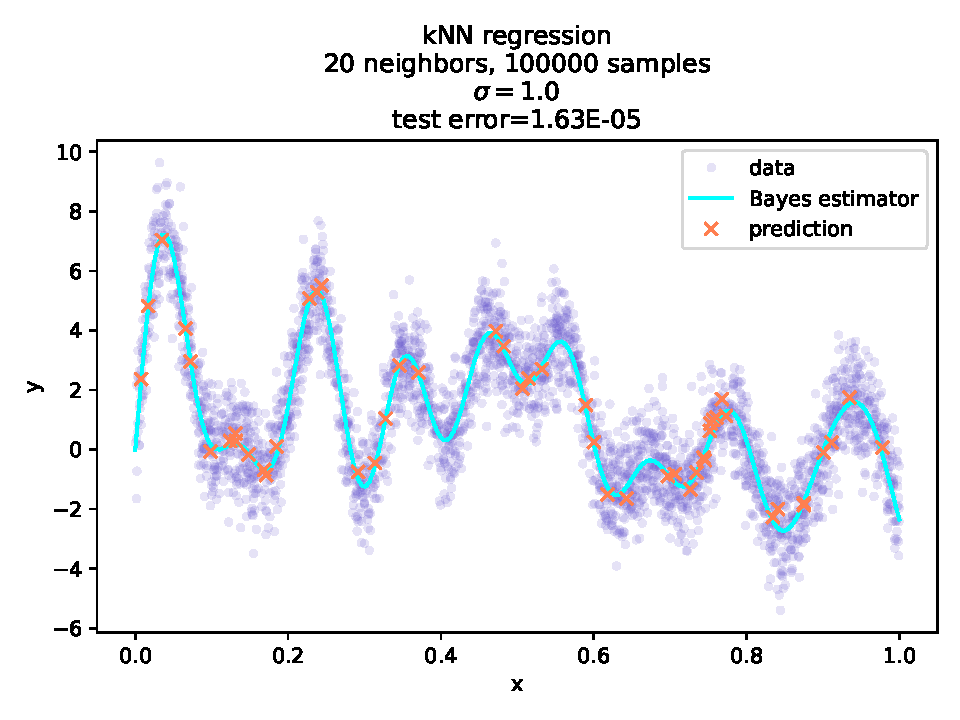
\includegraphics[width=0.7\textwidth]{images_1D/knn_k=20_samples=100000_sigma=1}
    	\label{fig:images_1D-kn}
    \end{figure}
\end{frame}


\begin{frame}

    The problem with local averaging is that the number of samples that we need in order to garantee a prediction error of order of magniture $\epsilon$ is

\begin{equation}
    n_{\epsilon} \geq \frac{\epsilon^{-d}d^{d/2}}{\alpha^{d/2}} 
\end{equation}

where $\alpha > $ is a constant. $n_{\epsilon}$ hence grows exponentially with
$1/\epsilon$, and this is an example of curse of dimensionality.

\end{frame}

\begin{frame}{Dimensionality reduction}
    \begin{itemize}
	\item Hence, in general, it is not possible to use local averaging when the input space dimension is larger than e.g. 20.
	\item \textbf{{However}}, often the data might actually occupy a \textbf{{subspace}} of lower dimension $q$, or it may be possible to project the data on such a subspace without loosing too much information.
	    \begin{itemize}
		\item Working in a subspace of lower dimension might speed up the algorithms.
		    \item It may also allow visualization of the data.
	    \end{itemize}
    \end{itemize}
\end{frame}

\begin{frame}{Methods of dimensionality reduction}
    \begin{itemize}
        \item \textbf{{feature selection}}: selecting a subset of the original dimensions.
	\item \textbf{{feature extraction}}: computing new features from the original features.
    \end{itemize}
\end{frame}




\section{Linear dimensionality reduction (Principal component analysis)}
\frame{\tableofcontents[currentsection]}

\begin{frame}

    \url{https://scikit-learn.org/stable/modules/unsupervised_reduction.html} 

    \url{https://en.wikipedia.org/wiki/Principal_component_analysis} 

\end{frame}


\begin{frame}{Introduction}
    \begin{itemize}
	\item Principal Component Analysis is a linear dimensionality reduction method.
	\item It is based on statistical and geometrical considerations.
	\item It was invented by Pearson at the beginning of XXth century but is still used today.
	\item Applications include : 
	    \begin{itemize}
		\item dimensionality reduction
		\item noise filtering
		\item prediction
		\item general data visualization and analysis
	    \end{itemize}
    \end{itemize}
\end{frame}

\begin{frame}{Example}
    In this paper, astrophysicists use PCA in order to test a new star temperature prediction method \cite{Bermejo2013} 
    \begin{figure}[htpb]
        \centering
        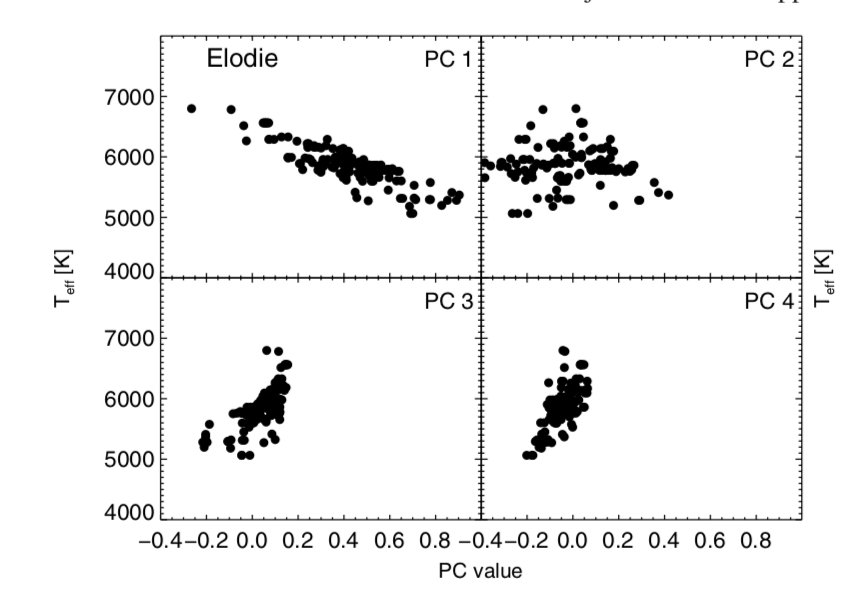
\includegraphics[width=0.65\linewidth]{temperature}
        \caption{PCA used in order to predict temperature.}
        \label{fig:temperature}
    \end{figure}
\end{frame}


\begin{frame}{Problem statement}
    \begin{itemize}
	\item We have multidimensional data.
    \end{itemize} 
    \begin{figure}[htpb]
        \centering
        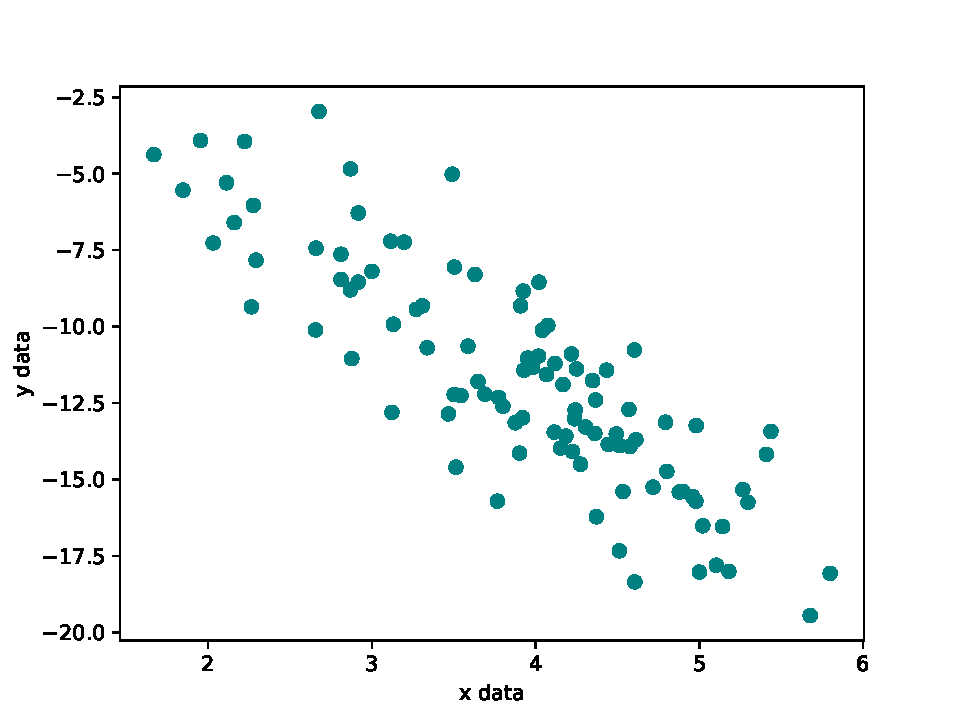
\includegraphics[width=0.8\linewidth]{pca_data}
	\caption{Data we want to analyze}
        \label{fig:pca_data}
    \end{figure}
\end{frame}

\begin{frame}{Problem statement}
    \begin{itemize}
	\item We have multidimensional data.
    \end{itemize} 
    \begin{figure}[htpb]
        \centering
        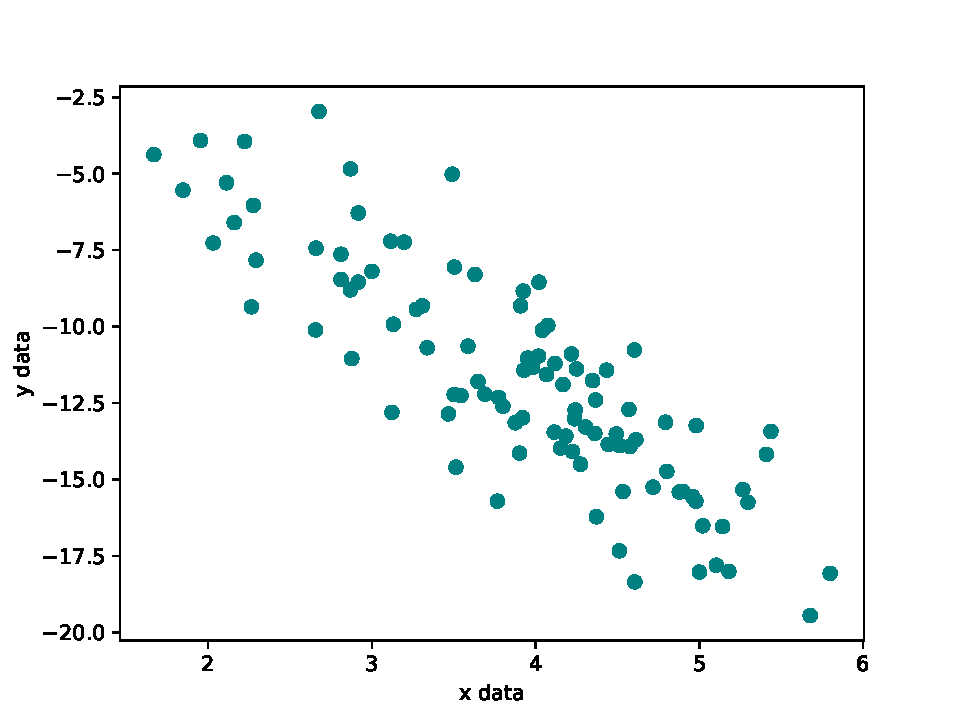
\includegraphics[width=0.4\linewidth]{pca_data}
        \label{fig:pca_data}
    \end{figure}
    We look for the axes that "explain" or carry the most variations in the data.

    Thoses axes will be called the \textbf{{principal components.}} 
\end{frame}

\label{sec:orthogonal_projection}

\begin{frame}{Visual intuition}
    \begin{figure}[htpb]
        \centering
        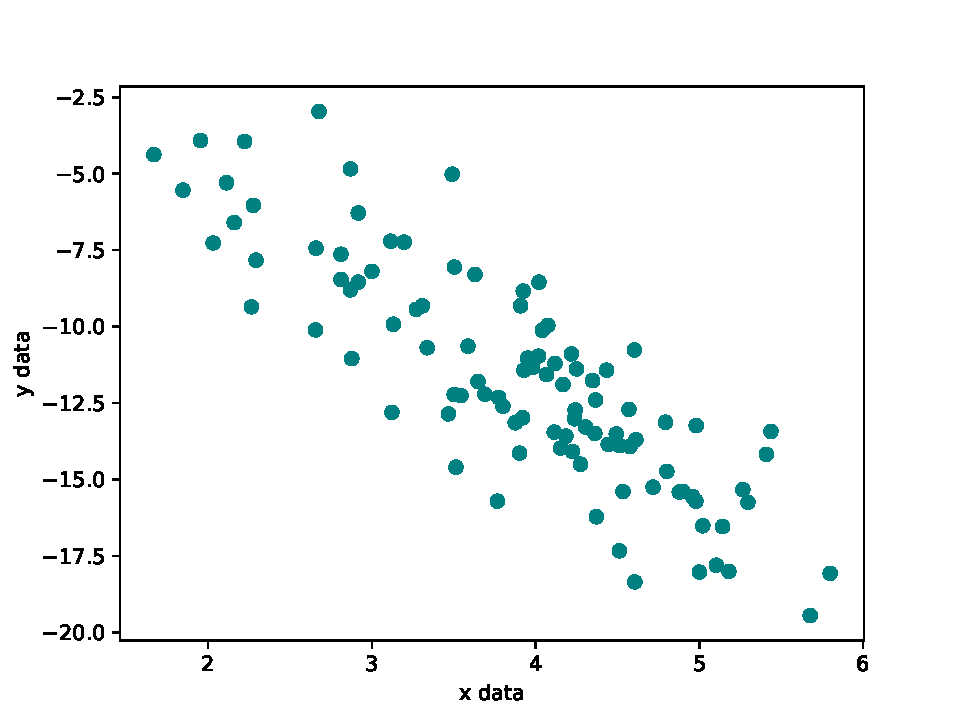
\includegraphics[width=0.6\linewidth]{pca_data}
        \label{fig:pca_data}
    \end{figure}
    When looking at this image, what axis would you suggest in order to carry the biggest variation among the data ?

\end{frame}

\begin{frame}{Formalization}
    We need a \textbf{{mathematical criterion}}  in order to formalize this intuition.

    In the case of a larger problem with more dimensions, it will not be possible to use visual feedback in order to choose the principal components (the axis).

    Furthermore, even in 2D, using only visualization, we can only do a \textbf{{approximation}} of the most relevant axis.
\end{frame}

\begin{frame}{Orthogonal projections}
   We will restate the problem in a mathematical way, using tools coming from \textbf{{linear algebra.}}  

    In particular, the concept of \textbf{{orthogonal projection}} is essential.
\end{frame}

\begin{frame}{Orthogonal projection}
   \begin{figure}[htpb]
       \centering
       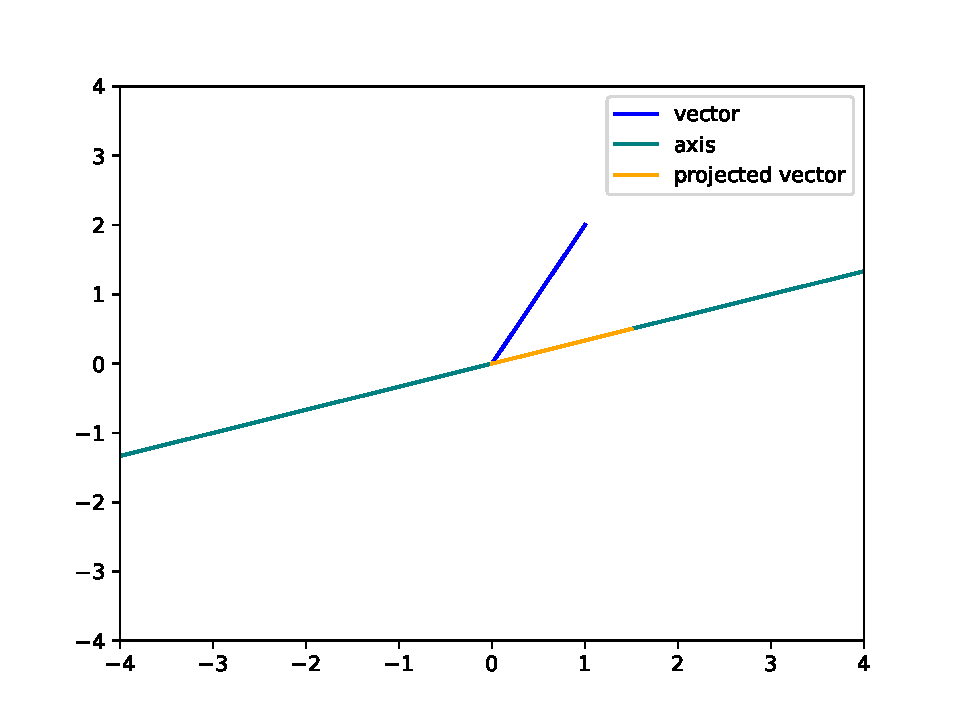
\includegraphics[width=0.6\linewidth]{projection}
       \label{fig:projection}
   \end{figure} 
   \exercice{\textbf{Mathematical problem}}
   Can you link orthogonal projections to the problem of finding the most relevant axis ?
\end{frame}

\begin{frame}{Inertia}
    \begin{itemize}
        \item The \textbf{{inertia}} related to an axis will be a measure of the quality of an axis.
	\item If $x_i$ is a sample from $n$ samples, and $\Delta$ an axis, we call $p_{x_i\rightarrow \Delta}$ the orthogonal projection of $x_i$ on the axis $\Delta$.
	\item The inertia related to $\Delta $ is:
	    \begin{equation}
		I_{\Delta}= \frac{1}{n} \sum^{n}_{i=1} d^2(x_i, p_{x_i\rightarrow \Delta})
	    \end{equation}
    \end{itemize}
\end{frame}

\begin{frame}{Inertia}
    \exercice{\textbf{No inertia}}

    In what situations could we have $ I_{\Delta}=0$ ?
\end{frame}

\begin{frame}{Inertia}
    \begin{figure}[htpb]
        \centering
	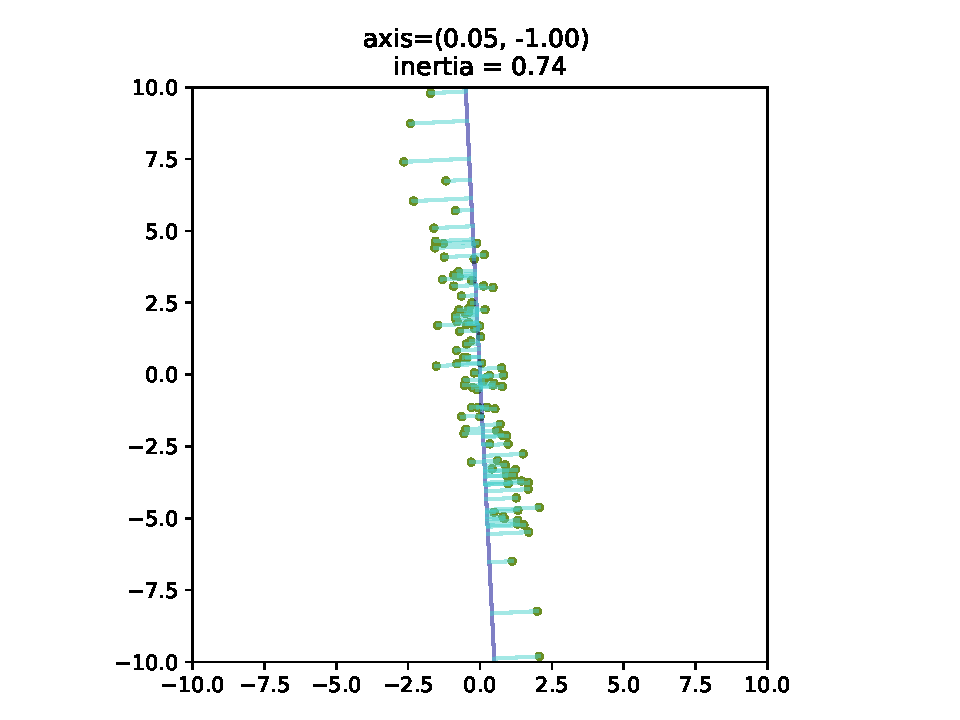
\includegraphics[width=0.8\linewidth]{A}
        \label{fig:projection axis=(0.95, 0.32)}
    \end{figure}
\end{frame}

\begin{frame}{Inertia}
    \begin{figure}[htpb]
        \centering
	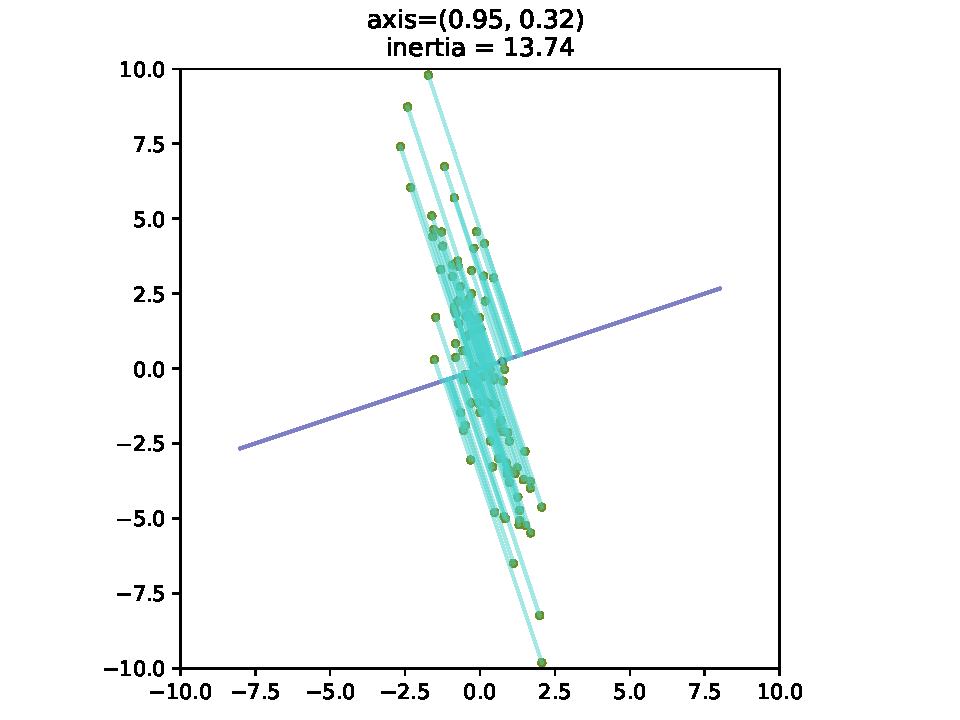
\includegraphics[width=0.8\linewidth]{C}
        \label{fig:projection axis=(0.45, -0.89)}
    \end{figure}
\end{frame}

\begin{frame}{Inertia}
    \begin{figure}[htpb]
        \centering
	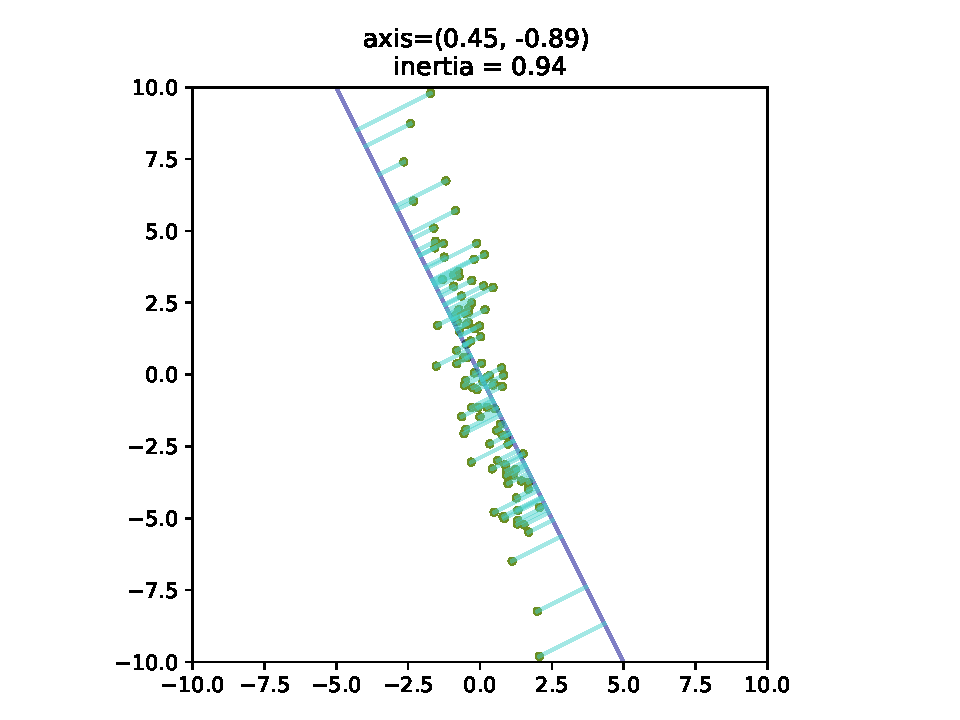
\includegraphics[width=0.8\linewidth]{B}
        \label{fig:projection axis=(0.05, -1.00)}
    \end{figure}
\end{frame}

\begin{frame}{Inertia}
    \exercice{\textbf{Computing an inertia}}

    \textbf{{cd day\textunderscore 4/1\textunderscore pca/toy\textunderscore data/}} and use the file \textbf{{inertia.py}} in order to represent the projections of the data onto a chosen axis and to compute the inertia of this axis.

    You need to add the computation of the inertia to the script (starting at line 75).

    What is your optimal axis ?
\end{frame}

\begin{frame}{Remark}
    Minimizing $I_{\Delta}$ is the same as maximizing $I_{\Delta^{*}}$ where $\Delta^{*}$ is the supplementary orthogonal space.
\end{frame}

\begin{frame}{Several principal components}
    \begin{itemize}
	\item In $2D$ (like in the former example), we  have at most $2$ principal component.
	\item However, when the data have more dimensions, it is possible to have \textbf{{several principal components}} (as many as the dimensionality of the data).
	\item the data are then projected on these components.
    \end{itemize}
\end{frame}

\begin{frame}{Link with expected values}
    There is a connection between the inertia and the \textbf{statistical variance} of a specific random variable.

    \begin{figure}[htpb]
    	\centering
    	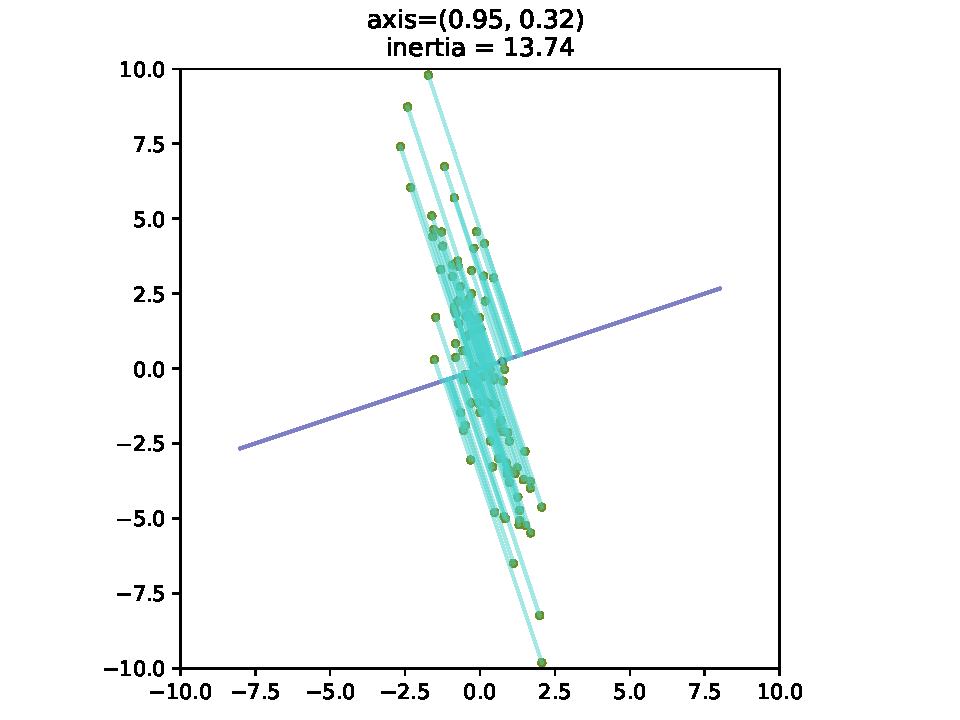
\includegraphics[width=0.5\textwidth]{C}
    	\label{fig:}
    \end{figure}
\end{frame}

\begin{frame}{Expected value (espérance)}
   \begin{itemize}
       \item For a discrete random variable $X$ that takes the values $x_i$ with probability $p_i$: 
	   \begin{equation}
	       E(X)= \sum^{n}_{i=1} p_ix_i
	   \end{equation}
       \item For a continuous random variable $X$ with density p(x): 
	   \begin{equation}
	       E(X)= \int xp(x)dx
	   \end{equation}
	\item Variance:
   \begin{equation}
       var(X) = E\Big(\big(X-E(X)\big)^2\Big)
   \end{equation}
   \end{itemize} 
\end{frame}

\begin{frame}{Probability vs Statistics}

    {\color{Purple}(Advanced notions)}

\begin{itemize}
    \item from a dataset of samples $(x_1, \dots, x_n)$, we can only compute \textbf{{statistics}} 
    \item for instance 
        \begin{itemize}
            \item sample mean:
                \begin{equation}
                    \hat{x} = \frac{1}{n} \sum^{n}_{i=1} x_i
                \end{equation}
            \item unbiased sample variance: 
                \begin{equation}
                    \frac{1}{n-1} \sum^{n}_{i=1} (x_i-\hat{x})^2
                \end{equation}

                The $ \frac{1}{n-1} $ factor instead of $ \frac{1}{n} $
                requires some theory to be properly understood.

        \end{itemize}
\end{itemize}
\end{frame}

    
\begin{frame}{Optimization with analytic solution}
    \begin{itemize}
        \item In practical applications, algorithms or analytic solutions are used in order to find the optimal axes.
        \item Methods include the \textbf{{Lagrange multiplier method}}
        \item The method shows that we need to compute the
            \textbf{{eigenvectors}}  of the \textbf{{covariance matrix.}} 
        \item {\color{Purple}See also: Gram matrix, power iteration algorithm}
    \end{itemize}
\end{frame}

\begin{frame}{PCA with scikit-learn}
    \begin{itemize}
 	\item \url{https://scikit-learn.org/stable/modules/decomposition.html} 
 	\item \url{https://scikit-learn.org/stable/modules/generated/sklearn.decomposition.PCA.html} 
    \end{itemize}
    We can use \textbf{{pca\textunderscore sklearn.py}} in order to find the principal components on the dataset of the previous exercise, using scikit-learn.
\end{frame}

\begin{frame}{Iris dataset}
     We can also perform PCA on the iris dataset as in the file \textbf{{1\textunderscore pca/iris/iris\textunderscore pca.ipynb}}.
    \begin{figure}[htpb]
        \centering
        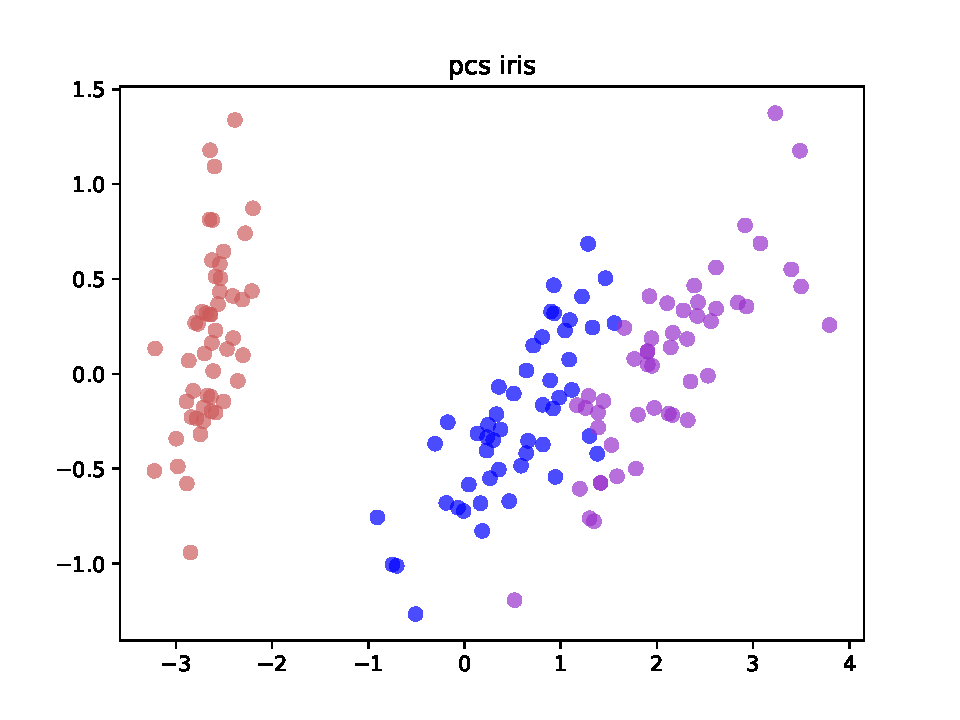
\includegraphics[width=0.6\linewidth]{pca_iris}
	\caption{PCA performed on the iris dataset. We see that the principal components are (almost) able to separate the 3 classes.}
        \label{fig:pca_iris}
    \end{figure}
    
\end{frame}

\begin{frame}{PCA on digits}
    \begin{itemize}
	\item We can apply PCA to the digits dataset, in \textbf{1\textunderscore pca/digits/}, using \textbf{pca\textunderscore digits.py}
    \end{itemize}
    \begin{figure}[htpb]
        \centering
        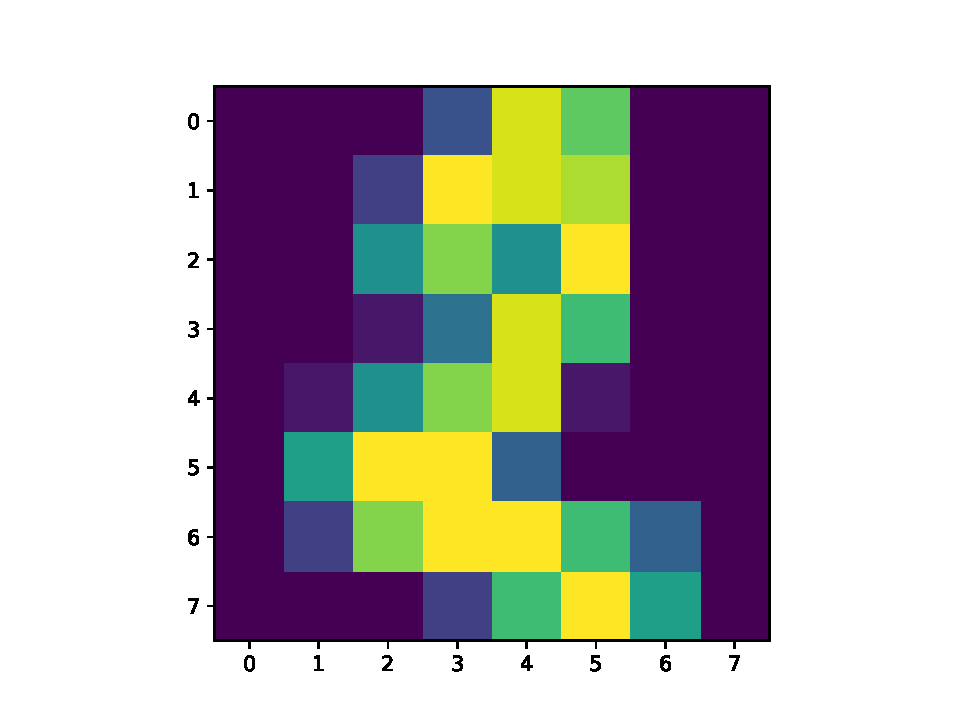
\includegraphics[width=0.5\linewidth]{sample_2}
        \label{fig:digits}
    \end{figure}
\end{frame}

\begin{frame}{PCA on digits}
    \begin{figure}[htpb]
        \centering
        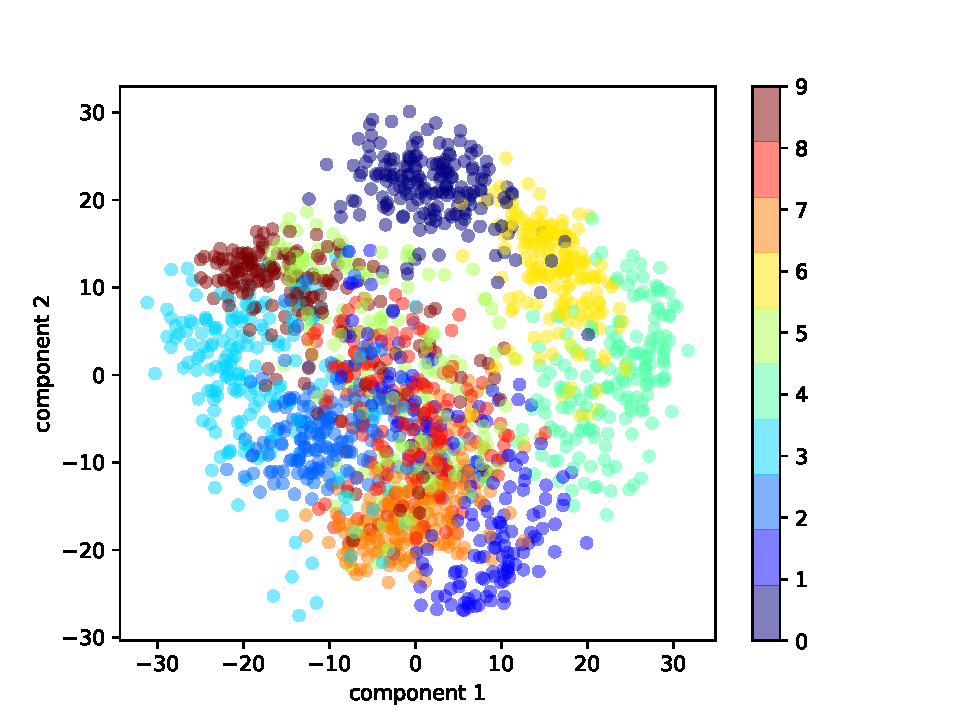
\includegraphics[width=0.8\linewidth]{projected_digits}
        \label{fig:projected_digits}
    \end{figure}
\end{frame}

\begin{frame}{Number of components}
    \exercice{\textbf{Choosing the number of components}}
    \begin{itemize}
    	\item The number of kept components for PCA is the most important hyperparameter. 
	\item Use the file \textbf{{pca\textunderscore digits\textunderscore variance.py}} in order to determine how many components are necessary in order to keep 75$\%$ of the variance in the digits dataset.
    \end{itemize}
\end{frame}

\begin{frame}{Number of components}
    \begin{figure}[htpb]
        \centering
        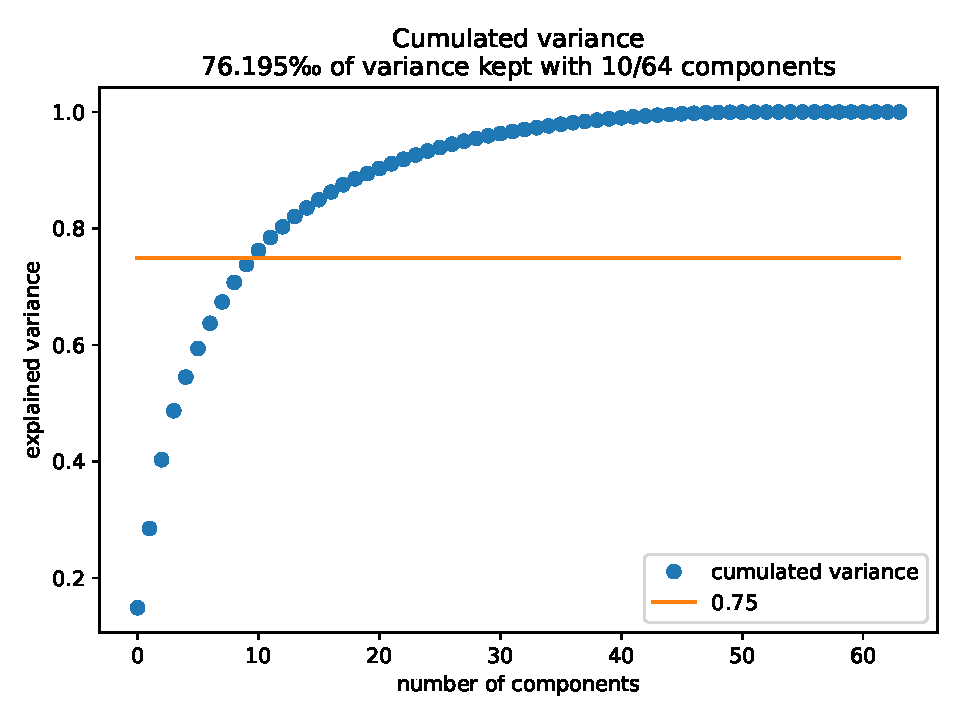
\includegraphics[width=0.7\linewidth]{explained_variance_ratio}
        \label{fig:explained_variance}
    \end{figure}
\end{frame}

\begin{frame}{Reconstruction}
\begin{figure}[htpb]
    \centering
    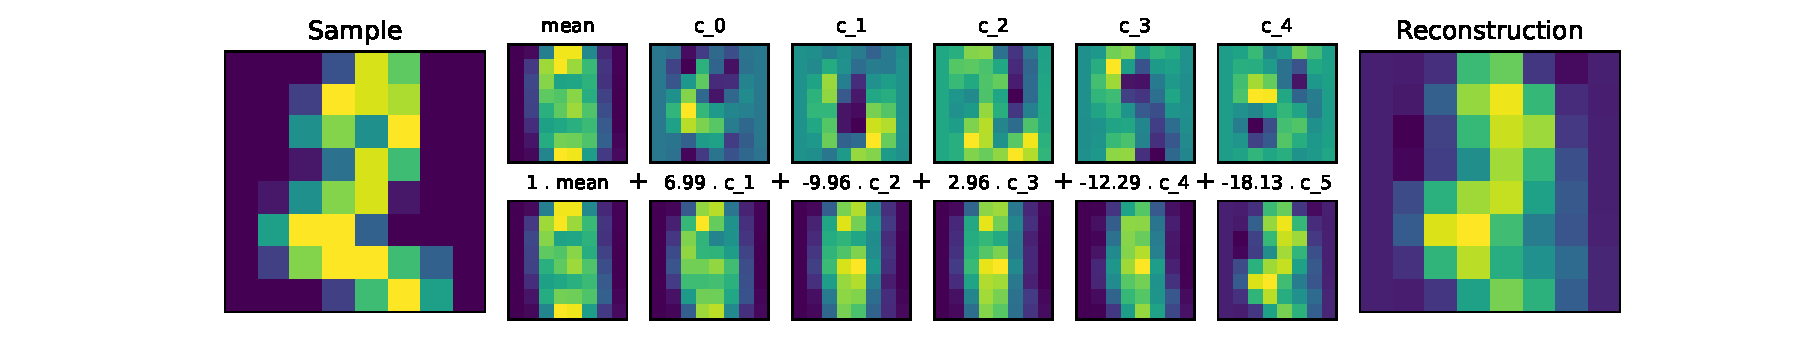
\includegraphics[width=0.8\textwidth]{sample_2_5_components}
    \caption{Reconstruction of a sample with 5 components}
    \label{fig:}
\end{figure}
\end{frame}

\begin{frame}{Reconstruction}
\begin{figure}[htpb]
    \centering
    
\includegraphics[width=0.8\textwidth]{sample_2_20_components}
    \caption{Reconstruction of a sample with 20 components}
\end{figure}
\end{frame}


\begin{frame}{Number of components}
    \exercice{\textbf{Redundancy}}

    What happens with the data contained in \textbf{{redundancy/redundant\textunderscore data.npy}} ? You can analyze them with the file \textbf{{redundancy/pca\textunderscore variance.py}}.
    
\end{frame}

\begin{frame}{Number of components}
   \begin{figure}[htpb]
       \centering
       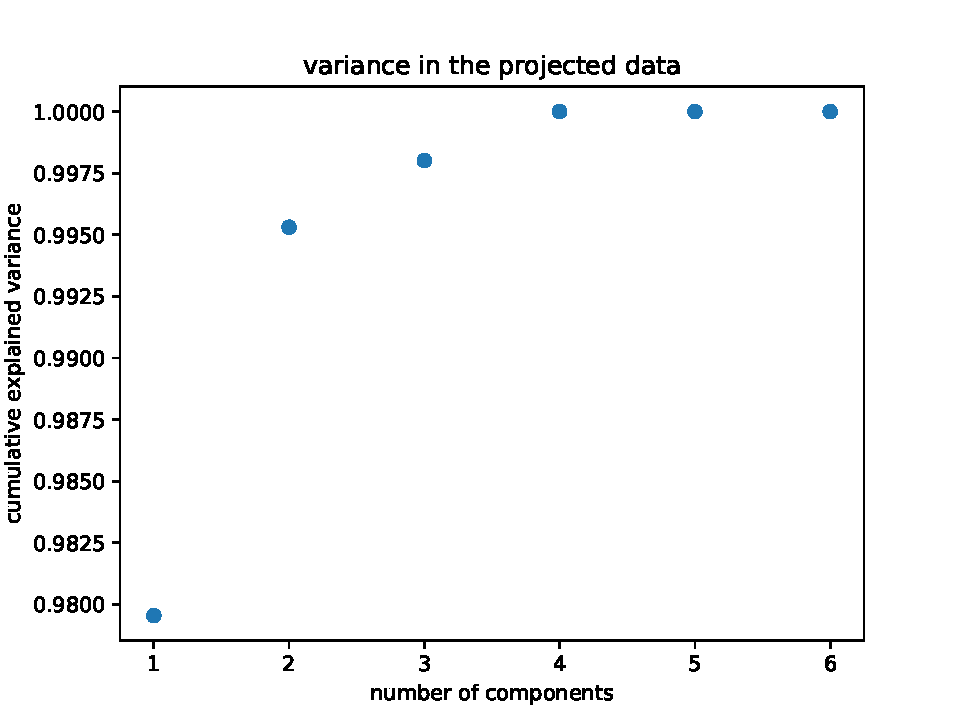
\includegraphics[width=0.8\linewidth]{explained_variance_redundancy}
       \label{fig:explained_variance_redundancy}
   \end{figure} 
\end{frame}

\begin{frame}{Number of components}
    \textbf{{Conclusion: }} PCA can help detemine whether some components carry no information in the data.
    
\end{frame}

\begin{frame}{Shortcomings of PCA}
   PCA is sensitive to :  
    \begin{itemize}
        \item outliers
	\item initial data scaling
	\item Many variants and heuristics exist on this topic.
    \end{itemize}
\end{frame}


\begin{frame}{Asset of PCA}
    Reducing the dimensionality of the data might be very helpful in a situation where you need to train a supervised algorithm on the projected data. The algorithm might be way faster on data that live in a smaller space. However, a sufficient amount of information should be kept during the reduction, hence the necessity of experimentation and knowledge of heuristics.
    
\end{frame}

\begin{frame}

    \url{https://scikit-learn.org/stable/auto_examples/cluster/plot_kmeans_digits.html} 
\end{frame}


\section{Nonlinear dimensionality reduction (manifold learning)}
\frame{\tableofcontents[currentsection]}

\begin{frame}

    \url{https://scikit-learn.org/stable/modules/manifold.html} 

    \url{https://en.wikipedia.org/wiki/Nonlinear_dimensionality_reduction} 

\end{frame}

\begin{frame}{Manifolds}
    \textbf{{Fundamental hypothesis (as before):}}

    In some cases, altough the dimensionality of the data is high (as for images), the data lie on a specific subpart of the linear space containing them.
\\

    This "subpart" is assumed to be a \textbf{{manifold}} (variété).
    
\end{frame}

\begin{frame}{Manifolds}
   \begin{figure}[htpb]
       \centering
       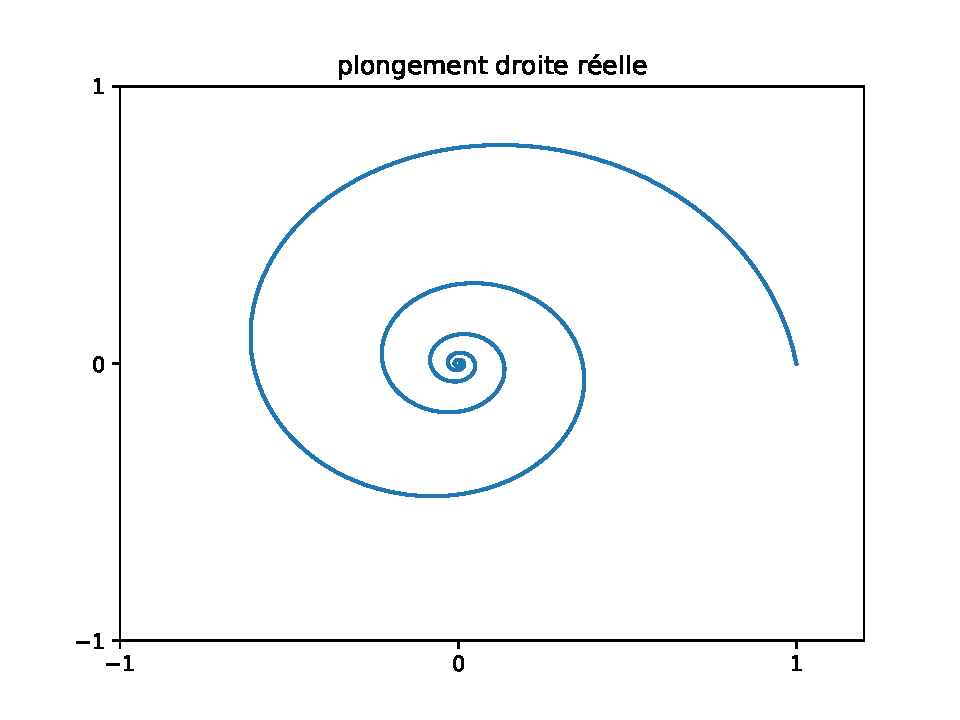
\includegraphics[width=0.7\linewidth]{plongement}
       \caption{1 dimensional manifold, in $ \mathbb{R}^2$ }
       \label{fig:plongement}
   \end{figure} 
\end{frame}

\begin{frame}{Linearity}
   \begin{itemize}
       \item In the case of PCA, the manifolds are \textbf{{linear subspaces}} of the ambient space : PCA is a \textbf{{linear method}} and does \textbf{{linear projections.}} 

	\item A linear mapping in a linear space $E$ is a mapping $u$ such that 
	    \begin{equation}
		\forall x, y \in E, u(x+y)=u(x)+u(y)
	    \end{equation}
   \end{itemize} 
\end{frame}

\begin{frame}{Nonlinearity}
    \begin{itemize}
	\item However, in many situations, the data might lie on \textbf{{nonlinear}}  manifolds.
	\item \textbf{{Manifold learning}} is the unsupervised learning of these manifolds in order to study the structure of the data.
    \end{itemize}
\end{frame}


\begin{frame}{Multidimensional scaling (MDS) / Positionnement multidimensionnel}
    \begin{itemize}
        \item Projects the data in a smaller subspace trying to preserve
            pairwise similarities between points.
    \end{itemize}
\end{frame}


\begin{frame}{t-SNE}
    \begin{itemize}
        \item t-Stochastic Neighbor Embedding \cite{VanDerMaaten2008}
        \item \url{https://lvdmaaten.github.io/tsne/} 
    \end{itemize}
\end{frame}

\begin{frame}{t-SNE on MNIST}
    \begin{figure}[htpb]
        \centering
        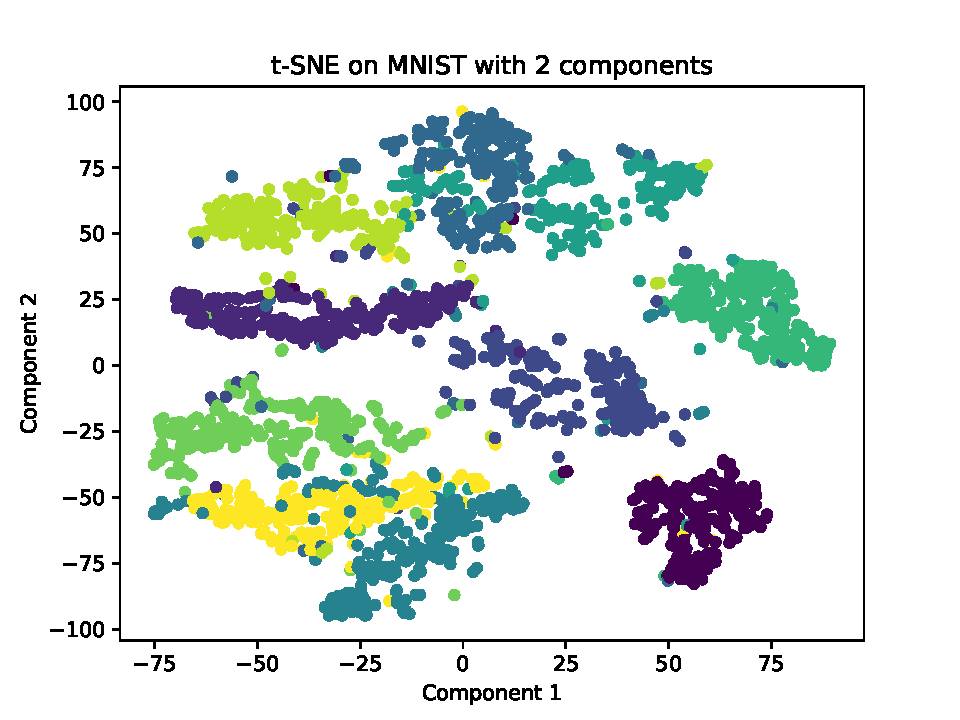
\includegraphics[width=0.7\linewidth]{t_SNE_2_components}
        \label{fig:tsne}
    \end{figure}
\end{frame}


\begin{frame}{ {\color{Purple}Seel also}}
    \begin{itemize}
        \item {\color{Purple}Isomap}
        \item {\color{Purple}LLE}
    \end{itemize}
\end{frame}


\begin{frame}{Comments}
    Some disadvantages of non linear manifold methods:
    \begin{itemize}
	\item  Hard to determine a good output dimension (whereas in PCA we can use explained variance) and it is hard to interpret the embedded dimensions (whereas in PCA we know what they mean).
	\item Depends on the number of neighbors chosen (if relevant)
	\item Often compuationally slower.
    \end{itemize}
\end{frame}


\begin{frame}
\frametitle{References}
\bibliographystyle{apalike}
\bibliography{pca.bib} 
\end{frame}

\end{document} 
